\documentclass[a4]{article}
\usepackage[utf8]{inputenc}
\usepackage[a4paper,top=3cm,bottom=2cm,left=3cm,right=3cm,marginparwidth=1.75cm]{geometry}
\usepackage{bm}
\usepackage{amssymb}
\usepackage{amsmath}
\usepackage{tikz}
\usepackage{geometry}
\usepackage{pgfplots} \pgfplotsset{compat=newest}
\usepackage{subcaption}
\usetikzlibrary{positioning}
\usetikzlibrary{intersections}
\usepackage[noadjust]{cite}
\renewcommand{\citedash}{--}   
\begin{document}
\title{Formal Verification of transcendental fixed and floating point algorithms using automatic theorem provers}
\maketitle

\normalsize
\begin{center}
\section*{Abstract}
\end{center}
We present a method for formal verification of transcendental hardware algorithms which shall scale to higher precision algorithms without suffering an exponential growth in runtimes. A class of implementations using piecewise polynomial approximation to compute the result is verified using MetiTarski, an automated theorem prover, which verifies a range of inputs for each call. The method was applied to commercial implementations from Cadence Design Systems with significant runtime gains over exhaustive testing methods and was even successful in detecting a bug in the one of the implementations.  

\section{Introduction}

Formal verification of floating point operations is becoming ever more challenging as hardware designs reach levels of complexity only previously seen in software. Its importance in industry is well known, highlighted by the Pentium floating point division bug \cite{pratt1995anatomy}. The bulk of this research was conducted during a research project at Cadence Design Systems and building on this I present a new approach to verification of floating point transcendental algorithms. It is expected that this technique will be viable for verification of high precision algorithms as there is evidence to suggest that runtimes will not scale exponentially with the precision. In this work I have focused on just implementations of the logarithm however the methodology can be applied to a wide range of algorithms. 

Traditional techniques rely on exhaustive testing of all inputs to verify such algorithms, but this can be resource intensive which may be prohibitive in some cases. The MPFR library is a C library for multiple-precision floating point computations with correct rounding \cite{fousse2007mpfr}, and is widely used as a reference for many verification tasks. For example some of the industrial implementations presented here were verified by comparing the outputs to the MPFR library and I shall demonstrate that the methodology used in this paper performed more efficiently. 


The paper will focus on implementations of transcendental functions in hardware which rely on piecewise polynomial approximations. In floating point arithmetic, the upper most portion of the input mantissa is passed to a lookup table which outputs a number of coefficients, the remainder of the input is then used to compute a polynomial approximation to the exact result. Scaling to handle the exponent is often computed in a separate section of the code. Such an approach is easy to verify using the methodology described in this paper but will hold for any implementation where it is possible to abstract an underlying mathematical model that can be expressed as a system of inequalities for verification purposes.

To produce the required proofs we use MetiTarski, an automatic theorem prover \cite{akbarpour2010metitarski} for real valued analytical functions, such as cosine and logarithm. It's a combination of a resolution theorem prover and a decision procedure for the theory of real closed fields which together allow it to prove polynomial inequalities. The inbuilt axioms are primarily upper and lower bounds on a set of supported functions which are obtained from their Taylor expansion or continued fraction expansions, for example:
$$\frac{1}{2} \leq x \leq 1 \Rightarrow \frac{x-1}{x} \leq ln(x) \leq \frac{3x^2-4x+1}{2x^2}$$

Conjectures are passed to MetiTarski in the form of a set of inequalities which are transformed by replacing any special function by an appropriate bound. Typically proofs are found in a few seconds \cite{akbarpour2009applications}, but if MetiTarski is unable to prove a conjecture it does not mean that the conjecture is false. For verification it is important that MetiTarski produces machine readable proofs which include algebraic simplification, decision procedure calls and resolution rules \cite{denman2009formal}. Amongst the various automated theorem provers MetiTarski is well suited because it supports high precision approximations to transcendental functions such as logarithm, cosine and sine. It also takes problems in the format of a sequence of inequalities to be proven with variables in a user defined range. My initial research inspired a new enhancement to MetiTarski and this paper contains the first application of this latest update. It is expected that this enhancement will simplify the verification procedure via this methodology and also reduce runtimes with some further development. 

\section{Related work}
John Harrison conducted some of the earliest work on floating point algorithm verification via theorem proving which relied on mechanical provers \cite{harrison1997floating}.Such an approach was labour intensive and not easily adaptable to changes in the algorithm, for example an increase in the input bit width would require a large portion of the work to be recomputed. However this laid the foundations in this area and with the development of sophisticated automatic provers can be built upon more efficiently here. An important problem for this methodology will be the interplay of floating point and bit level operations as is common in real code \cite{mine2012abstract}. For example computing $2^n$ in double precision can be found by shifting $n+1023$ left by 52 bits which is computationally efficient and cheap. Such techniques make verification more challenging particularly in the context of high precision transcendental functions \cite{lee2016verifying} as SMT theories are insufficient. 

For verification of small floating point functions the Gappa tool \cite{de2006assisted,boldo2009combining} has been testes and is still being developed. Gappa uses interval arithmetic in order to prove conjectures whilst MetiTarski relies on cylindrical algebraic decomposition to generate proofs. Both methods are valid but for some problems interval arithmetic is substantially weaker. Hopefully this study may prove useful to compare the two different underlying processes in verification applications in the future.

\section{Hardware Models}
In this paper I present a method to verify designs which rely on making piecewise polynomial approximations to transcendental functions \cite{tang1991table,strollo2011elementary,pineiro2005high}. The input to the function is typically in floating point format \cite{goldberg1991every} which stores a number in the format: $(-1)^{s} \times 2^{e-b} \times 1.significand$, where in IEEE 754 standard single precision s is a single bit representing the sign, the exponent e is an 8 bit integer, the bias b is a constant equal to 127 and the significand is 23 bits long. The class of design verified in this paper are minor variants on the following high level description which employs a k bit lookup table and a degree m polynomial approximation:
\begin{enumerate}
\item The top k bits of the significand are passed to a lookup table which outputs some coefficients $a_0,...,a_m$
\item The lower $23-k$ bits of the significand, say $x$, are used to compute\newline $a_0+a_1x+...+a_mx^m$
\item Scaling step computed to account for the exponent
\end{enumerate} 
Where k and m are some integers dependent upon the implementation. Step 3 will vary depending upon the function to be implemented, for example for computing logarithm base 2 it will simply involve a series of adders. The verification methodology described here could be generalised to a wider class of algorithms for which it is possible to reduce the verification to checking a system of inequalities. 


\section{Verification Methodology}
Given a hardware implementation of a transcendental function following the template above we obtain an abstraction which is verifiable via MetiTarski. If as above, the top k-bits of the significand are passed to a lookup table, for a fixed exponent and signed bit we reduce the verification problem to just $2^k$ calls to MetiTarski. Therefore, the  full verification over all inputs is reduced to 
just $2^{k+8+1}$ MetiTarski conjectures to be proven. In some cases verification over all such inputs is not even necessary as a short hand proof may be able to prove the correctness of the results to handle exponent scalings. Of course, most verification tasks deploy massive parrelisation to reduce the run times, for example one verification problem may use 500 processors simultaneously and similar parrelisation may be used to reduce the runtimes in our approach as each conjecture passed to MetiTarski is completely independent. In nearly all commercial implementations k is relatively small as lookup tables require a large amount of space on a chip. Assuming our interpolation coefficients are stored in a readable file and are able to express the problem as a set of inequalities, the procedure follows the same basic outline.


\vspace{0.2cm}
\noindent\fbox{\begin{minipage}{\dimexpr\textwidth-2\fboxsep-2\fboxrule\relax}
\textbf{Procedure Outline:}
\begin{enumerate}
\item Write a template problem for the inequalities to be proven, with placeholders for all the relevant interpolation coefficients and upper bit values.
\item Use a wrapper script to read the coefficients and replace them in the template problem to generate the full set of MetiTarski problems.
\item Run the Perl script which accompanies MetiTarski to test all of the problems.
\item Refine error modeling on problems which are not proven.
\item Exhaustively test regions where MetiTarski was unsuccessful.
\end{enumerate}
\end{minipage}}
\vspace{0.2cm}


With this process I analyse a simple 'toy implementation' which is based on the outline given above for computing the natural logarithm which should demonstrate the methodology. The implementation takes as an input an 8 bit integer $x_0x_1...x_7$ and outputs an approximation to $\ln(1.x_0...x_7)$. The top four bits, $x_0..x_3$, are passed to a lookup table which returns the 10 bit interpolation coefficients $a, b, c$. Writing $x=0.x_0...x_7$ the approximation generated is:
$$ \overline{\ln(1+x)}=c + bx +ax^2 $$

This example is designed to be very simple to show the underlying principles of the verification methodology and later shall adapt this implementation so that it is more relevant to industrial implementations. In this case, the implementation is accurate to $2^{-10}$, which put formally states:
$$|\ln(1+x)-\overline{\ln(1+x)}|<2^{-10}\hspace{0.5cm} \forall \hspace{0.2cm} x= 0.x_0...x_7 $$
This can easily be verified using exhaustive testing as the input space is very small. MetiTarski is able to exactly model this implementation with no errors, so we generate a total of 16 problems for MetiTarski to prove which correspond to the values of the upper 4 bits of the input and determine the interpolation coefficients. For example the template MetiTarski problem for upper bits, $y=0.x_0...x_3$ and $X$ the value of the lower bits, would be:
$$ 0\le X \le 2^{-4}-2^{-8} \Rightarrow |\ln(1+y+X)-(c+b(y+X)+a(y+X)^2)|$$

Following the outline above with this template problem, all 16 problems are generated and the Perl script automates the MetiTarski calls. Therefore the only manual input required is to produce the template problem. MetiTarski is able to provide proofs for all of these problems with a total runtime of 5.3 seconds and no more than 0.3 seconds is spent on any one proof. Of course on such a small input space exhaustive search is quicker by several orders of magnitude, taking less than a 10$^{th}$ of a second, however as we shall see later our technique does not suffer from exponentially increasing runtimes as we increase the precision of our implementation.


With this basic understanding of the methodology I shall now adapt the 'toy implementation', because in commercial hardware engineers have constraints on area and performance targets to meet so they use techniques to reduce the resource requirements of the function. One of the main techniques used is to truncate bits throughout the algorithm which reduces the number of adders required and generally improves the performance, typically with some cost in terms of the accuracy of the approximation. In our implementation the impact on accuracy when using these techniques is quite significant but by choosing the points at which truncations are made more carefully the effect can be reduced. The new implementation returns an approximation of the form:  
$$ \overline{\ln(1+x)}=c + 2^{-8}\left \lfloor{b(x_0...x_7)}\right \rfloor +a(0.x_0...x_5)^2 $$

\noindent In this case the approximation is accurate to $2^{-7}$, which stated formally says: 
\begin{equation}
|\ln(1+x)-\overline{\ln(1+x)}|<2^{-7}\hspace{0.5cm} \forall \hspace{0.2cm} x= 0.x_0...x_7
\end{equation}
This is easily checked using exhaustive testing but notice that the implementation uses bit truncations on the 1st and 2nd order terms, which should mean that this algorithm returns an answer more quickly than the previous method. However, since MetiTarski has no understanding of the integers, such non-analytic functions are are difficult to model. Inspired by this research, Professor Larry Paulson explored the addition of support for a floor function. Due to the nature of the floor function it is difficult to provide good bounds so an axiom which simply states that $x-1< floor(x)\le x $ was added to MetiTarski. It should be noted that this bound is poor when the inputs under investigation are close to 1, as for example MetiTarski will fail to prove:
$$floor(\frac{1}{2})\geq 0$$
However for the toy model and other examples investigated in this paper such a bound is sufficient to verify the function to the same precision that can be verified via exhaustive testing. Therefore using this function it is possible to produce produce a MetiTarski conjecture where, now we allow X to be the integer value of the bottom 4 bits and y the integer value of the top 4 bits which determine the coefficients a, b, c as before:
\begin{equation}
0\le X \le 15 \hspace{0.2cm} \Rightarrow \hspace{0.2cm}|\ln(1+2^{-4}y+2^{-8}X) - M_1\_\ln(1+x)|<2^{-7}
\end{equation}
where $$M_1\_\ln(1+x)=c+2^{-8}floor(b(X+2^{4}y))+a2^{-12}(floor(2^{-2}X+2^{2}y))^2$$

\noindent An alternative method to model the errors arising from such bit manipulations in the hardware implementations is to include additional error variables in place of the floor function. These techniques were explored before support for the floor function was included so we can compare both methodologies. Modeling our updated implementation using error variables rather than the floor function would yield a MetiTarski problem of the form:
$$0\le X \le 15 \hspace{0.1cm} \& \hspace{0.1cm} 0\le \epsilon_1<1\hspace{0.1cm} \& \hspace{0.1cm} 0\le \epsilon_2<1 $$
\begin{equation}
\Rightarrow |\ln(1+2^{-4}y+2^{-8}X) - M_2\_\ln(1+x,\epsilon_1,\epsilon_2)|<2^{-7}
\end{equation}
where
$$M_2\_\ln(1+x,\epsilon_1,\epsilon_2)=c+2^{-8}(b(X+2^{4}y)-\epsilon_1)+a2^{-12}((2^{-2}X+2^{2}y)-\epsilon_2)^2$$

Surprisingly for this particular problem using additional error variables rather than the floor function actually had minimal impact on the overall runtime for the 16 problems which was unexpected because MetiTarski runtimes are doubly exponential in the number of variables. However the floor function is a recent addition to MetiTarski, and we may be able to improve its performance by fine-tuning its heuristic parameters, which at present are at default values. On industrial implementations however, it was necessary to manually combine error variables and estimate a bound on how large these could be. This was often very challenging as some of the error variables were highly correlated so using the floor function in general makes the process of generating a template problem significantly simpler. Unfortunately during the initial bulk of this work the floor function was not supported and using error variables was the only available option.

To illustrate why this technique is powerful I extend the implementation above to larger input spaces, where the approximation made is essentially the same, using the same coefficients and lookup table, just where our input now may be 10 bits rather than 8 bits for example. Figure \ref{runtime_graph} shows a comparison of how the runtimes of the two verification methods changes as the input space grows. Notably the MetiTarski method has roughly constant runtimes, which is not unexpected because MetiTarski is an analytic tool so increasing the space of discrete inputs doesn't really affect the MetiTarski problems. Whereas exhaustive testing suffers from an exponential growth, although it should be noted this is a slightly unfair comparison as in reality for commercial implementations the size of the lookup table will increase with the input space. An increase in the lookup table will affect the MetiTarski runtimes as the number of problems will grow however as we shall see in the results that follow there is still a significant gain.
\begin{figure}
\centering
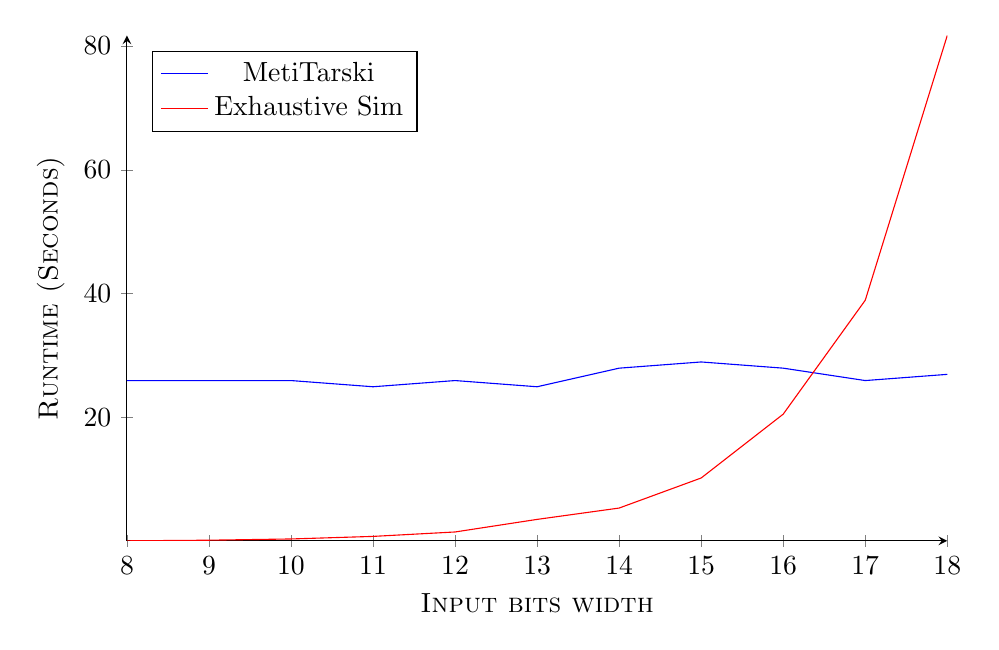
\begin{tikzpicture}
\begin{axis}[
    axis lines = left,
    xlabel = \textsc{Input bits width},
    ylabel = \textsc{Runtime (Seconds)},
    legend pos=north west,height=80mm, width=120mm]

\addplot[
    color=blue,
    ]
    coordinates {(8 ,26)(9 ,26)(10,26)(11,25)(12,26)(13,25)(14,28)(15,29)(16,28)(17,26)(18,27)   };
    \addlegendentry{MetiTarski}
\addplot[color=red,
        ]
        coordinates{(8 ,0.14548254013061523 )
(9 ,0.24578046798706055 )(10,0.4463155269622803  )
(11,0.8605005741119385  )(12,1.574721336364746   )
(13,3.603602409362793   )(14,5.432856559753418)
(15,10.283031702041626)(16,20.580944299697876)
(17,38.95604610443115)(18,81.67475938796997)

 };
        \addlegendentry{Exhaustive Sim}
\end{axis}
\end{tikzpicture}

\caption{A graph demonstrating the runtime comparison of the competing verification procedures on implementations of growing precisions. \label{runtime_graph}
}
\end{figure}
Even if MetiTarski is unable to prove all the problems passed to it, if it is able to prove some of them then at least the range of the input space upon which we need to do exhaustive testing is reduced. In the following section we shall demonstrate a situation where this technique would have been relevant. 

\section{Applications}
In this section we present some results from applying this methodology to the verification of several larger commercial implementations. For intellectual property reasons it is not possible to describe the particular implementations in detail but the runtime results can be found in table \ref{result} and demonstrates that the technique has real world relevance. 

The single precision floating point $\log_2$ was a release candidate for Cadence Design Systems which takes as inputs 32 bit floating point numbers and outputs in the same format. This was the first test case studied using the MetiTarski verification methodology and previously the implementation had been checked using a basic benchmarking tool. Through our investigations, a bug was discovered in the code such that for a small input region it broached the claimed error bound. The region was identified by first using the methodology described above to verify inputs in the region $[0.5,2)$, then because the exponent scaling for $\log_2$ simply involves adding the exponent to the approximation made on the $1.significand$ component a hand proof was sufficient to complete the verification. However the proof identified a region in which the exponent addition breached the accuracy claimed and exhaustive testing on this region identified a large number of counter examples in this region. For the purpose of testing the methodology we exhaustively tested all inputs and as predicted everywhere but this narrow region the implementation met its accuracy claim.

The second implementation in table \ref{result} was an experimental test case generated primarily to analyse how the MetiTarski method performed on higher precision algorithms. It takes as input a fixed point number with 8 bits before the decimal place and 24 bits after, so the total number of possible inputs is $2^{32}$ but it is a higher precision algorithm and is far more accurate using a larger lookup table.


\begin{center}
\begin{table}[h!]
\centering
\begin{tabular}{ |c|c|c| } 
\hline
 Design & Single precision floating point $\log_2$ & Fixed point 8.24 $\log_2$    \\
\hline
 Input Region Verified& $[0.5,2)$ & $[1,2) $ \\ 
 \hline 
 MetiTarski Problems & 128 & 512 \\
 \hline
 MetiTarski Runtime &  7 minutes & 4 minutes \\ 
 \hline
 Exhaustive Test Runtime & 42 minutes & 53 minutes \\ 
\hline
\end{tabular}
\caption{Verification runtime results for industrial implementations of logarithm base 2, results obtained running on a single core}
\label{result}
\end{table}
\end{center}
The results show that the speedup achieved by MetiTarski is significant on the single precision logarithm but notably the speedup for the higher precision experimental implementation was greater. Such an observation combined with the above data would suggest that this methodology could be viable verification of higher precision hardware where traditional exhaustive techniques will fail. 


\section{Conclusion}
Using the methodology described above we successfully verified a variety of fixed and floating point logarithm implementations and even identified a bug in a near production algorithm. Most interesting are the runtime results which provide stong evidence to suggest that this technique will be viable in the future when higher precision algorithms are developed. For a set of algorithms following a basic template it is possible to automate the whole verification procedure after the intial template and wrapper scripts are written, so in such a setting the technique is quite powerful. 

However in addition to the above results, attempts were made to verify a more complex algorithm using this methodology which was less successful as the manual effort required was too great. This is where the technique is most challenging and is perhaps its greatest flaw. Generating the initial template problem is a non trivial task, as the verification engineer needs to understand the design implementation and model the errors accordingly. A simpler error model may be used initially to establish whether the algorithm is correct to a higher error rate initially, but to obtain a full proof several refinements of the model might be required, keeping into account the different errors introduced and their correlation. Therefore it has limited scope and the verification engineer requires a very strong understanding of the hardware to produce a full verification. One additional step to the methodology could be the use of a binary chopping technique applied to the input region of each problem. If successful, this would allow the engineer to further reduce the input space on which exhaustive testing is neccessary. For implementations which follow a standard model and particularly bespoke higher precision implementations the methodology shows promise and perhaps should be the subject of greater research.
\bibliographystyle{plain}
\bibliography{bibliography.bib}


\end{document}
